\documentclass[12pt]{article}
\parindent=0.25in

\setlength{\oddsidemargin}{0pt}
\setlength{\textwidth}{440pt}
\setlength{\topmargin}{0in}
\usepackage{amssymb}
\usepackage{amsfonts}
\usepackage{amsmath}
\usepackage{cancel}
\usepackage{latexsym}
\usepackage[center]{subfigure}
\usepackage{epsfig}
\usepackage{3952}
\usepackage{3952-thm}
\usepackage{pstricks,pst-node,pst-tree}
\usepackage{soul, xcolor}
\usepackage{bbold}
\usepackage[backref, colorlinks,citecolor=blue,bookmarks=true]{hyperref}  

\pagestyle{headings}    % Go for customized headings

\newcommand{\handout}[5]{
   \noindent
   \begin{center}
   \framebox{
      \vbox{
    \parbox[t]{4in} {\bf #1 } \vspace{3mm}  {\hfill \bf #2 }
       \vspace{2mm}
       \hbox to 6.00in { {\Large \hfill #5  \hfill} }
       \vspace{1mm}
       \hbox to 6.00in { {\it #3 \hfill #4} }
      }
   }
   \end{center}
   \vspace*{1mm}
}

\hypersetup{linkcolor=magenta}

\begin{document}

\handout{MATH 3952 (Undergraduate Seminar): Quantum Information Theory}{Spring 2024}
{Organizer: Patrick Lei; Presenter: Chloe Lambert}
{Scribe: Mark Chen}{Lecture 6, Talk 1: March 4, 2024}

\thispagestyle{plain}
% \setcounter{section}{-1}
\section*{Chapter 6: Bell's Theorem}
\section{Hidden Variables}
Recall that incompatible operators cannot both be measured deterministically (measuring one for sure means not being able to measure the other deterministically, with the product of the standard deviations of the two is explicitly lower bounded by $\left|\frac{1}{2i}\langle[A,B]\rangle\right|$).\\

\noindent This is something that Albert Einstein felt unnpleasant about. Albert Einstein, Boris Podolsky, and Nathan Rosen argued in their 1935 paper that the reason why one of the two incompatible states must be indeterminant is that:
\begin{itemize}
    \item First of all, both have definite values for the same qubit at the same time.
    \item Secondly, it's just that we only have knowledge of one of them at a time (``\textbf{hidden variable}" in the sense that it is present in nature but not accounted for in the theory).
\end{itemize}

\noindent It was until 1964, when John Bell showed that the \textbf{local hidden variable} hypothesis can be tested and \underline{refuted}. Then, there are other specific theories to also refute some specific types of hidden-variable theories:
\begin{itemize}
    \item Bell's theorem: to refute \textbf{local hidden-variable} theories.
    \item Kochen-Spcker theorem: to refute \textbf{non-contextual hidden-variable} theories.
    \item Pusey-Barret-Rudolph theorem: to refute \textbf{preparation independent hidden-variable} theories.
\end{itemize}
So, if any hidden-variable theory does exist, it has to be \textbf{non-local, contextual, and preparation independent}.

\begin{definition}[Locality]
Things can only be directly affected by their surroundings (so what seems to be happening with quantum entanglement should not be happening at distance faster than speed of light).
\end{definition}

\begin{definition}[Contextuality]
Can be seen as a direct generalization of non-locality, by Fine's theorem. It talks about how results of measurements depend on the commutator of the observable being measured, i.e. on its ``context." 
\end{definition}

\begin{definition}[Preparation Independence]
If we independently prepare two quantum states, then their hidden variables are also independent.
\end{definition}

\section{Quantum Correlations}
This more formally discusses something we mentioned before: given two entangled states, how accurately can we separate them?

\begin{definition}[Quantum Correlation]
A mathematical description of how \underline{correlations} \underline{between measurements of physical properties} in quantum systems can be \underline{quantified} (note that this is the most meaningful for entangled states). 
\end{definition}

\begin{definition}[Singlet]
A quantum system is a singlet if all qubits involved are entangled. For example, all the Bell states are singlets.
\end{definition}

\noindent Recall that:
\begin{itemize}
    \item For some entangled state, say $\Ket{\psi} = \Psi^- = \frac{1}{\sqrt{2}}\prt{\Ket{01} - \Ket{10}}$, we have $$
    \kb{\psi}{\psi} = \frac{1}{4}(\mathbb{1}\otimes \mathbb{1} - \sigma_x \otimes \sigma_x - \sigma_y \otimes \sigma_y - \sigma_z \otimes \sigma_z)
    $$
    \item Recall that, for $A$ and $B$ which are single-qubit observables with eigenvalues $\pm 1$, we can write them as $$
    \begin{aligned}
        A &= \vec{a}\cdot \vec{\sigma}
        B &= \vec{b}\cdot \vec{\sigma},
    \end{aligned}
    $$ where $\vec{a}, \vec{b}$ are unit vectors on a three-dimensional Euclidean space.
\end{itemize}

\begin{fact}\label{fact:eigenvalues-of-A-tensor-B}
\noindent Then, we can write $A\otimes B = (\vec{a}\cdot \vec{\sigma}) \otimes (\vec{b}\cdot \vec{\sigma})$, so the eigenvalue of $A\otimes B$ is the product of the eigenvalues of $A$ and $B$ (which are both $\pm 1$ as we already mentioned). So, the eigenvalue of $A\otimes B$ is:
\begin{itemize}
    \item ($+1$) when the outcomes of $A$ and $B$ agree (both $1$ or both $-1$).
    \item ($-1$) when the outcomes of $A$ and $B$ disagree (one with $1$ and the other with $-1$).
\end{itemize}
\end{fact}

\begin{definition}[Expected value of $A\otimes B$]\label{def:exp-value-A-tensor-B}
Now, we have two ways to calculate such an expected value:
\begin{itemize}
    \item (Directly use fact \ref{fact:eigenvalues-of-A-tensor-B}) $$
        \langle A\otimes B \rangle = 1\cdot \Pr[\text{outcomes of $A$ and $B$ agree}] + (-1) \cdot \Pr[\text{outcomes of $A$ and $B$ disagree}]
    $$
    \item (By definition) For expected value of $A\otimes B$ in state $\Ket{\psi}$: $$
    \begin{aligned}
    \langle A\otimes B \rangle
        &= \Bra{\psi} A\otimes B\Ket{\psi}\\
        &= \Trace{(\vec{a}\cdot\vec{\sigma})\otimes (\vec{b}\cdot\vec{\sigma})\underset{\frac{1}{4}(\mathbb{1}\otimes \mathbb{1} - \sigma_x \otimes \sigma_x - \sigma_y \otimes \sigma_y - \sigma_z \otimes \sigma_z)}{\underbrace{\kb{\psi}{\psi}}}} \\
        &= -\frac{1}{4}\Trace{(\vec{a}\cdot \vec{\sigma})\sigma_x \otimes (\vec{b}\cdot \vec{\sigma})\sigma_x + (\vec{a}\cdot \vec{\sigma})\sigma_y \otimes (\vec{b}\cdot \vec{\sigma})\sigma_y + (\vec{a}\cdot \vec{\sigma})\sigma_z \otimes (\vec{b}\cdot \vec{\sigma})\sigma_z}\\
        &= -\frac{1}{4}\Trace{4(\vec{a}\cdot \vec{b})\mathbb{1}\otimes \mathbb{1}}\text{, \hl{because $(\vec{a}\cdot \vec{\sigma})\sigma_k = 2a_k,k\in \{x,y,z\}$}}\\
        &= - \vec{a}\cdot \vec{b}
    \end{aligned}
    $$

    \textbf{Some analysis:} If $A$ and $B$ choose the same observable, $\vec{a} = \vec{b}$, then the expected value of $\langle A\otimes B \rangle$ is $-1$, meaning they will \textit{always} have the opposite outcome.
\end{itemize}
\end{definition}

\begin{definition}
Based on different values of $\langle A\otimes B\rangle\in [-1, 1]$, we have:
\begin{itemize}
    \item ($\langle A\otimes B\rangle=-1$) \textbf{Perfect anti-correlation}.
    \item ($\langle A\otimes B\rangle=0$) \textbf{No correlation}.
    \item ($\langle A\otimes B\rangle=1$) \textbf{Perfect correlation}.
\end{itemize}
\end{definition}

\section{CHSH Inequality \& Bell's Theorem}
CHSH is the initials of the names of the authors of the 1969 paper that theorized this inequality. The idea is simple, starting from the following set-up:
\begin{itemize}
    \item We have Alice and Bob.
    \item Each of the has a choice of selecting from two measurements. $A_1$ and $A_2$ for Alice, and $B_1$ and $B_2$ for Bob. Each of the $A_1, A_2, B_1, B_2$ is a random variable that can take up a value of $\pm 1$.
    \item Then, we can define a new quantity called the \textbf{CHSH quantity}: $$
    S := A_1B_1 + A_1B_2 + A_2B_1 - A_2B_2,
    $$ where the last term has $-1$ coefficient, because we want to have the condition where three pairs of the four possible pairs of $A_kB_k$ to be $1$ (meaning their values agree) and one of the possible pairs to be $-1$ (meaning their values disagree).
\end{itemize}

\noindent Now, the inequality goes as follows:
\begin{itemize}
    \item (Raw values argument) $$
    \begin{aligned}
    S
        &= A_1B_1 + A_1B_2 + A_2B_1 - A_2B_2
        &= A_1(B_1 + B_2) + A_2(B_1 - B_2),
    \end{aligned}
    $$ so that, regardless if $B_1$ and $B_2$ agree, one of the two terms on the two sides of the addition is $0$, and the other have $B_1\pm B_2 = \pm 2$. Then, since $A_1, A_2 = \pm 1$, the overall value is $$
    \boxed{S = \pm 2}.
    $$
    \item (Expected value) $$
    \begin{aligned}
    |\langle S \rangle|
        &= |\langle A_1(B_1 + B_2)\rangle + \langle A_2(B_1 - B_2)\rangle| \\
        &\leq 2.
    \end{aligned}
    $$ This is actually a simple argument: since $B_1 \pm B_2$ can only be one of $\pm 2$, and then, times a $\pm 1$, the absolute value of the product must be at most $2$.
\end{itemize}

\begin{remark}
Now, this is one of the proposed counter-argument to the \textbf{hidden variable} and \textbf{locality} requirements as Einstein raised, by proposing some conclusions to refute based on these assumptions. Particularly, the assumptions we used here are:
\begin{itemize}
    \item \textbf{(Hidden Variable)} All observable have definite values; it's just that we don't know them.
    \item \textbf{(Locality)} Outcomes of the measurements of Alice and Bob don't affect each other.
\end{itemize}
\end{remark}

\subsection{Bell's Theorem via CHSH}
Now, using the CHSH set-up, we introduce quantum theoretical things to it, i.e. we perform the aforementioned measurements but now on qubits instead (known as the \textbf{CHSH test or Bell test}).\\

\noindent Recall that we have $$
S = A_1\otimes (B_1 - B_2) + A_2\otimes (B_1 + B_2),
$$ using the same form as before. So, if the two qubits are in singlet state, then we have already seen from definition \ref{def:exp-value-A-tensor-B} that  $\langle A\otimes B\rangle = -\vec{a}\cdot\vec{b}$. So, if we set up $\vec{a_1}, \vec{a_2}, \vec{b_1}, \vec{b_2}$ as:
\begin{center}
    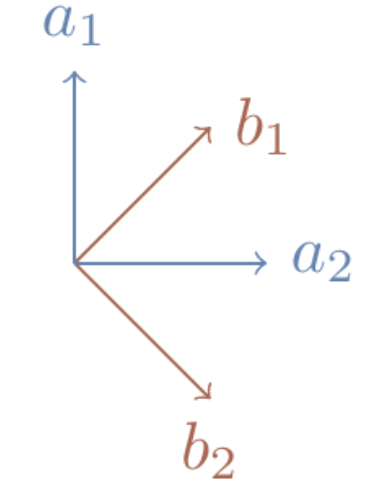
\includegraphics[width = 7em]{images/1.jpg}
\end{center}
We have $$
\begin{aligned}
    \langle A_1 \otimes B_1 \rangle = \langle A_2 \otimes B_1 \rangle= \langle A_2 \otimes B_2 \rangle &= \frac{1}{\sqrt{2}}\\
    \langle A_1 \otimes B_2 \rangle &= -\frac{1}{\sqrt{2}}
\end{aligned},
$$ which can be used to plug into $$
\boxed{\langle S\rangle =} \langle A_1\otimes B_1 \rangle - \langle A_1\otimes B_2\rangle +\langle A_2\otimes B_1 \rangle+\langle A_2\otimes B_2\rangle \boxed{= 2\sqrt{2}},
$$ which \hl{clearly exceeds the CHSH inequality limit of $2$}!

\begin{remark}
This violation of the proposed CHSH inequality based on \underline{Hidden Variable} and \underline{Locality} assumptions has been observed in many experiments! 
\end{remark}

\begin{theorem}[Bell's Theorem, Stated Compactly, Again]
The behavior of entangled quantum systems cannot be explained by \textbf{local hidden variables}. In other words, outcomes in quantum mechanics really are random, and it’s not simply our lack of knowledge about some background process.
\end{theorem}

\begin{remark}
If we can enforce \textbf{non-locality} in an experimental setup (for example, by ensuring that Alice and Bob are \underline{sufficiently far apart} so that there is not enough time between Alice making a measurement and Bob receiving his measurement result) then an experimental verification of the CHSH test proves to us that the system is behaving in an inherently \textbf{non-classical} and, importantly, \textbf{unpredictable manner}.\\

\noindent This means that this is a good test to see if our devices are performing as they are supposed to, and are untampered by any potential eavesdroppers. In other words, the CHSH test is key for \textbf{securing quantum protocols}. (*Note, on the contrary: If an eavesdropper has observed our system to the extent that they can predict out outcomes, then that very predictability means that there is a hidden-variable description of the system, and the CHSH inequality is not violated.)\\

\noindent A motto of this story, by Bell, ``If [a hidden-variable theory] is local it will not agree with quantum mechanics, and if it agrees with quantum mechanics it will not be local."
\end{remark}

\end{document}